\chapter{Działanie programu}
\thispagestyle{chapterBeginStyle}

\section{Instalacja}

Do poprawnego działania aplikacji wymagany jest system operacyjny wspierający zestaw bibliotek OpenGL. Rozważa się dwie możliwości instalacji:
\begin{enumerate}
\item Użycie pre-kompilowanego pliku wykonywalnego, skompilowanego na odpowiednią platformę.
\item Własnoręczna kompilacja przy użyciu polecenia 'make', przy czym należy spełnić następujące wymagania: 
	\begin{itemize}
	\item Kompilator g++ wspierający standard C++14
	\item Zainstalowane w systemie programistyczne biblioteki z zestawu OpenGL
	\item Zainstalowane w systemie programistyczne biblioteki z zestawu freeglut
	\item Narzędzie obsługujące pliki typu Makefile (np. linuxowy 'make')
	\end{itemize}
\end{enumerate}

\section{Dane wejściowe}

Wymagany jest przez aplikację zewnętrzny plik z opisem modelu w formacie {liczba1,liczba2,liczba3,\ldots}. Kolejne liczby oznaczają kolejne długości fragmentów, z których złożony jest model. Ścieżkę do wspomnianego pliku należy podać do standardowego wejścia programu. Po uruchomieniu plik wczytywany jest przez aplikację i następuje generowanie modelu.

\section{Poszukiwanie rozwiązywania}

Po poprawnym wygenerowaniu modelu następuje proces jego rozwiązywania. Ze względu na złożoność algorytmów może on potrwać od ułamka sekund aż do czasu bliżej nieokreślonego. Czas rośnie wraz ze złożonością modelu, tj. liczbą łączeń znaczących.

\section{Prezentacja wyniku}

Wynik przedstawiony jest w postaci interaktywnej animacji komputerowej.

Sterowanie klawiaturą:
\begin{itemize}
\item 'W' - przybliżenie modelu
\item 'S' - oddalenie modelu
\item 'N' - następny ruch
\item 'P' - poprzedni ruch
\end{itemize}

Obsługiwane są również zdarzenia pochodzące od myszy (touchpada, \ldots). Poruszanie myszą z przyciśniętym lewym klawiszem myszy daje możliwość obracania modelu pod dowolnym kątem. Dzięki temu użytkownik jest w stanie dokładnie przyjrzeć się modelowi zarówno w stanie spoczynku, jak i podczas wykonywania przez program obrotów.

\begin{figure}[h]
    \centering
    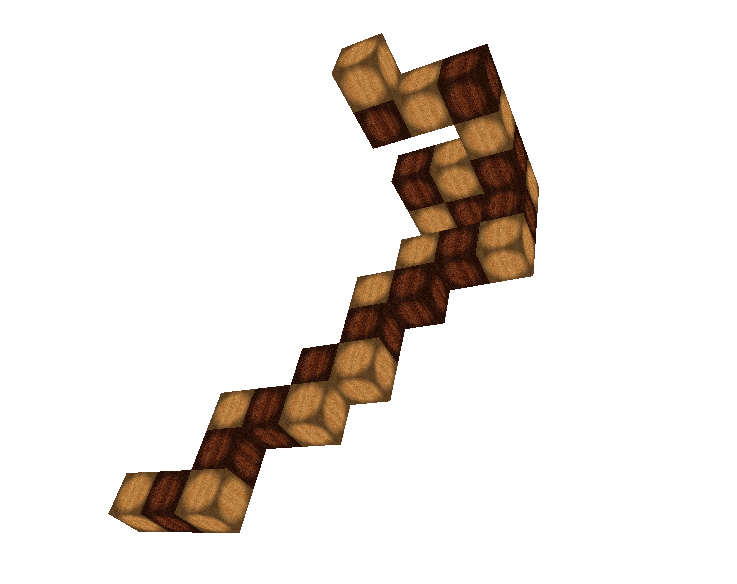
\includegraphics[width=0.7\textwidth]{using}
    \caption{Przykładowy zrzut ekranu wykonany w czasie działania programu}
    \label{fig:using1}
\end{figure}